\documentclass[a4paper,10pt]{article}
\usepackage[spanish]{babel}
\usepackage[utf8]{inputenc}
\usepackage[breaklinks=true]{hyperref}
\usepackage{verbatim}
\usepackage{amsmath}
\usepackage{graphicx}
\usepackage{subfig}
%\usepackage{subfigure}
\RequirePackage{fontawesome}
%opening

\begin{document}

\begin{titlepage}
\centering
{
\includegraphics[width=0.9\textwidth]{fing_uncuyo}\par}
\vspace{1cm}
{\bfseries\LARGE Universidad Nacional de Cuyo \par}
\vspace{1cm}
{\scshape\Large Facultad de Ingeniería \par}
\vspace{3cm}
{\scshape\Huge Predicción de Precios de Criptomonedas con ARIMA y Prophet \par}
\vspace{3cm}
{\itshape\Large Proyecto Final: Anexo III\\Inteligencia Artificial I \par}
\vfill
{\Large MOLINA, Mauro \par}
{\Large FLORES, Daniel Emiliano \par}
\vfill
{\Large Marzo 2022 \par}
\end{titlepage}

\newpage

\textbf{\large Gráficos de periodo mensual y semanal aleatorios con Prophet}
\begin{figure}[h!]
 \centering
  \subfloat[]{
   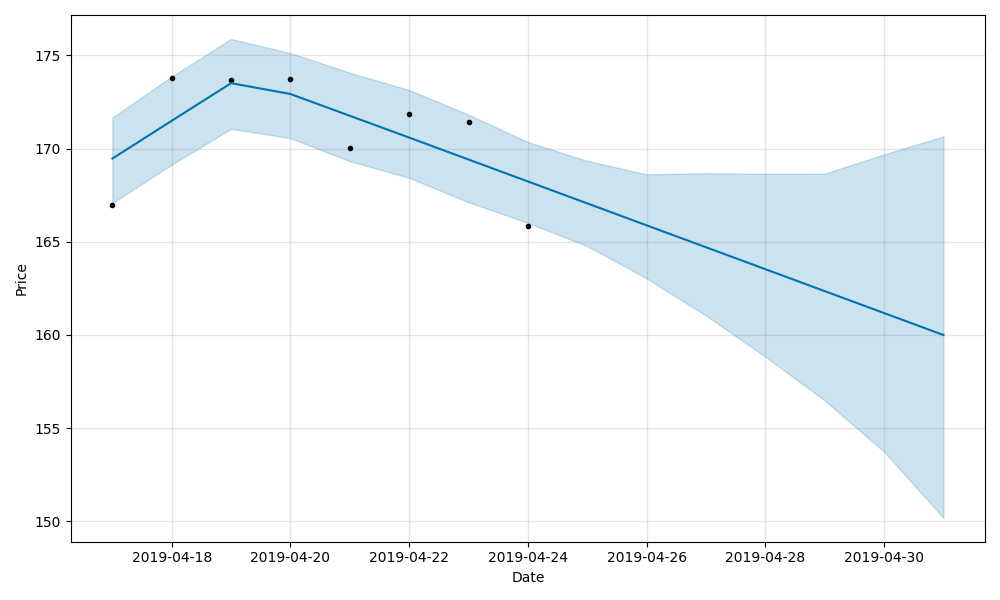
\includegraphics[width=0.5\textwidth]{./plots/prophet/eth/week/1}}
  \subfloat[]{
   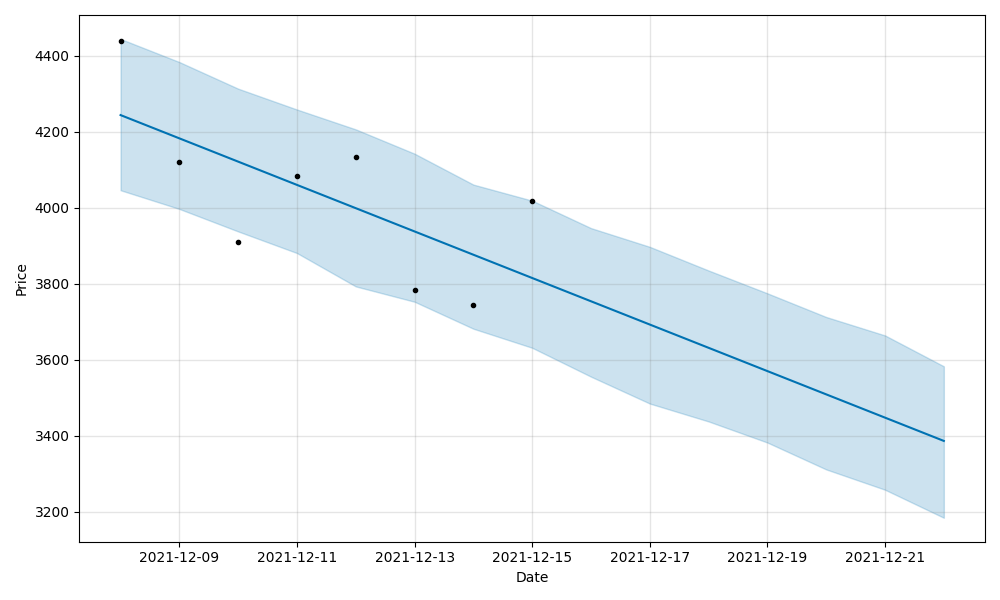
\includegraphics[width=0.5\textwidth]{./plots/prophet/eth/week/2}} \\
  \subfloat[]{
   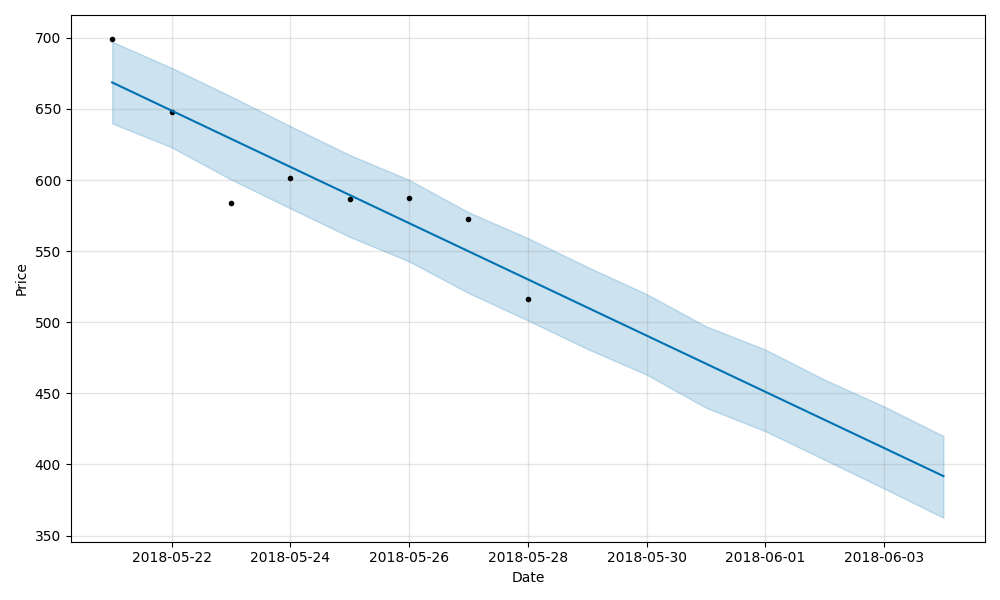
\includegraphics[width=0.5\textwidth]{./plots/prophet/eth/week/3}}
   \subfloat[]{
   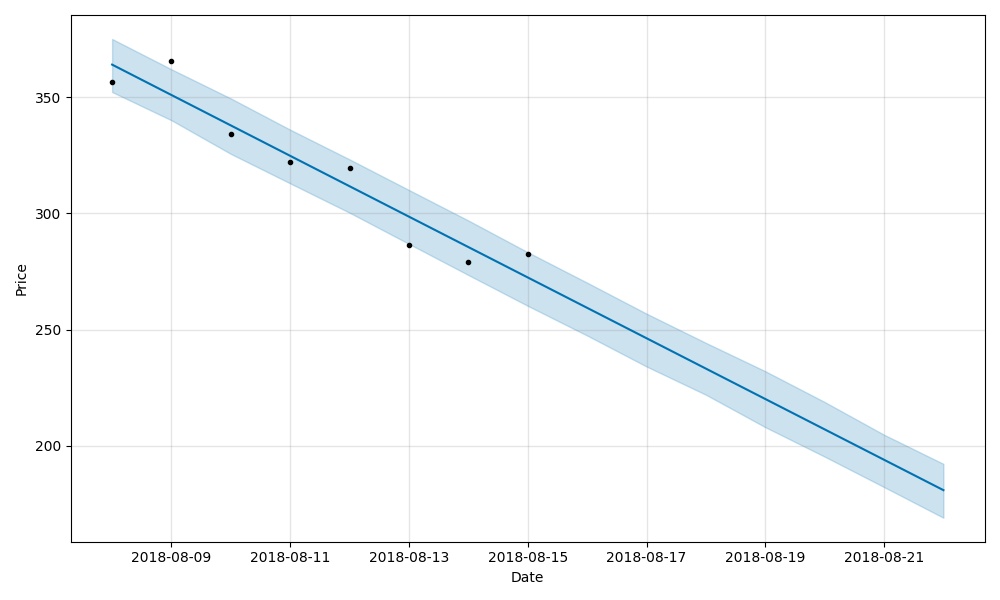
\includegraphics[width=0.5\textwidth]{./plots/prophet/eth/week/4}} \\
   \subfloat[]{
   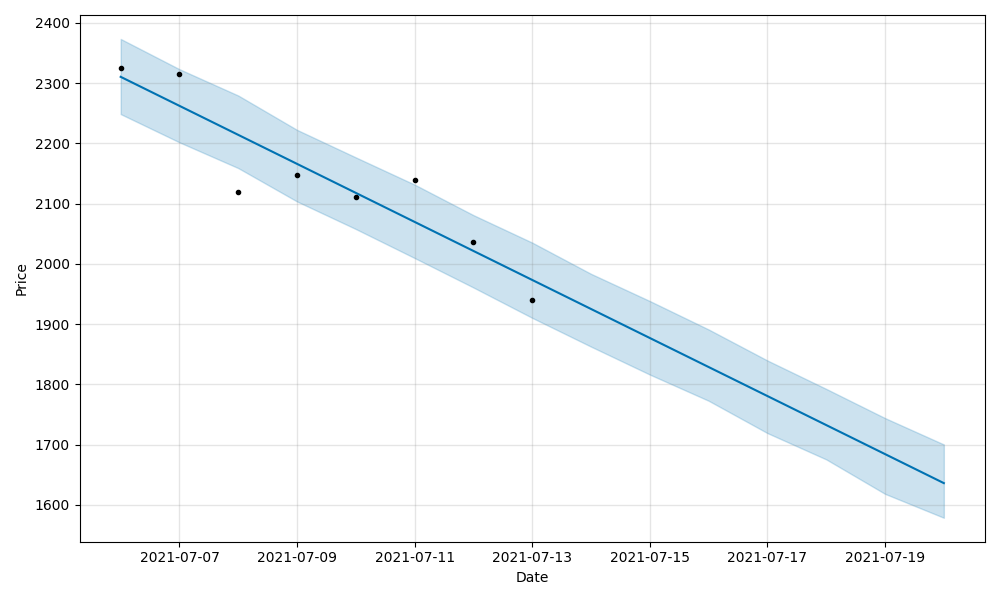
\includegraphics[width=0.5\textwidth]{./plots/prophet/eth/week/5}}
   \subfloat[]{
   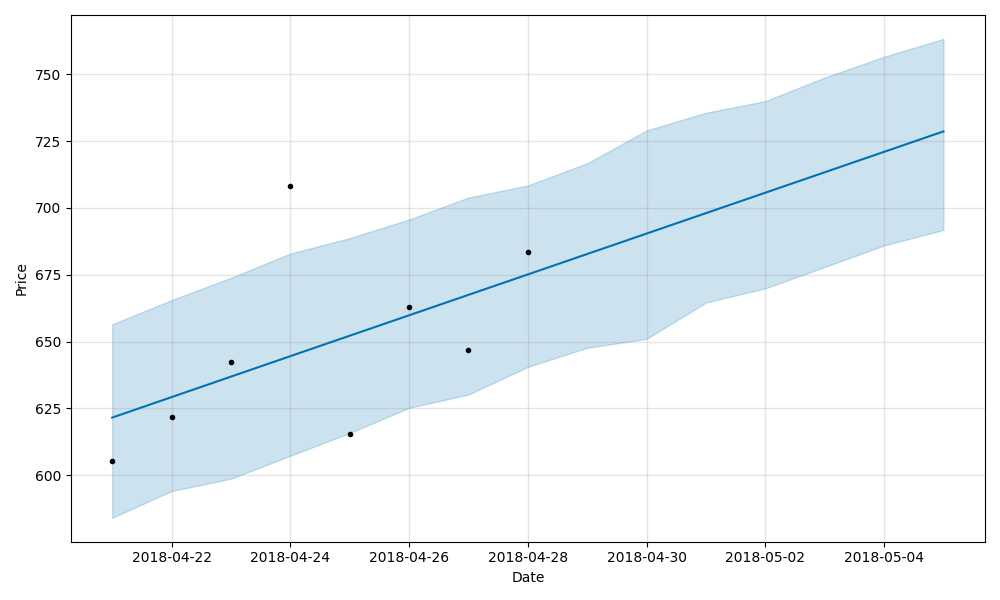
\includegraphics[width=0.5\textwidth]{./plots/prophet/eth/week/6}} \\
   \subfloat[]{
   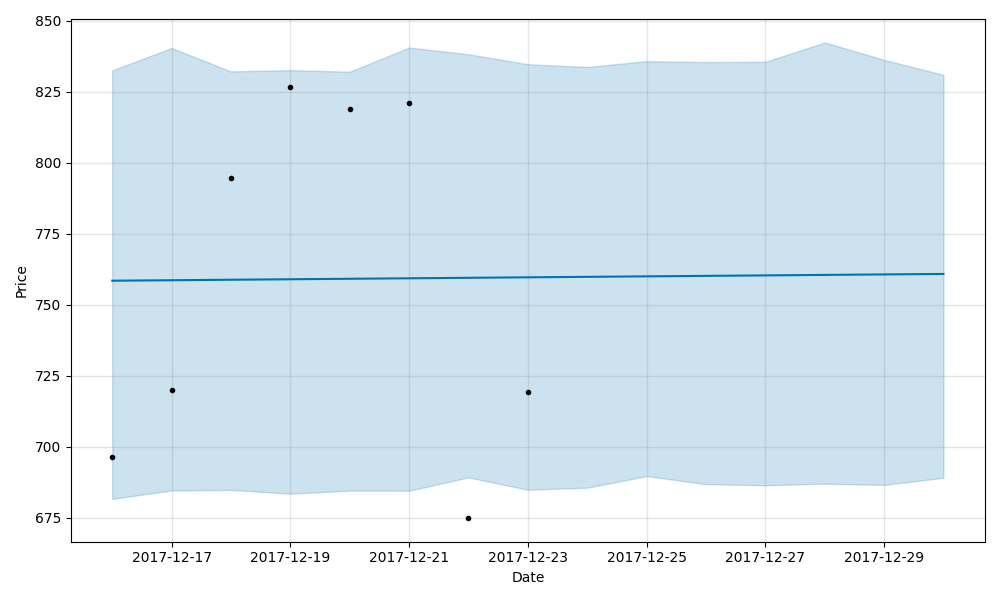
\includegraphics[width=0.5\textwidth]{./plots/prophet/eth/week/7}}
   \subfloat[]{
   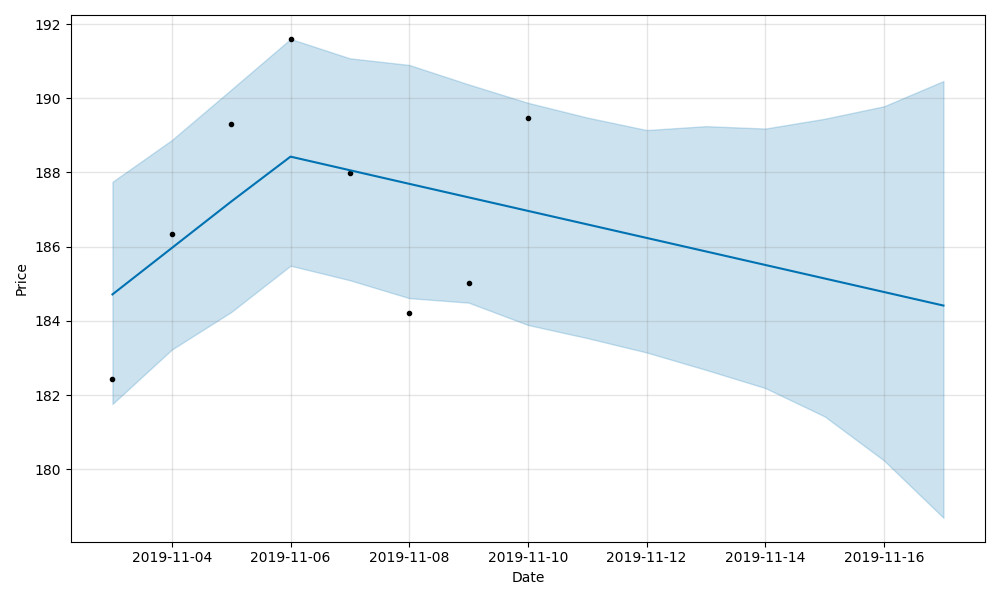
\includegraphics[width=0.5\textwidth]{./plots/prophet/eth/week/8}} \\
   \subfloat[]{
   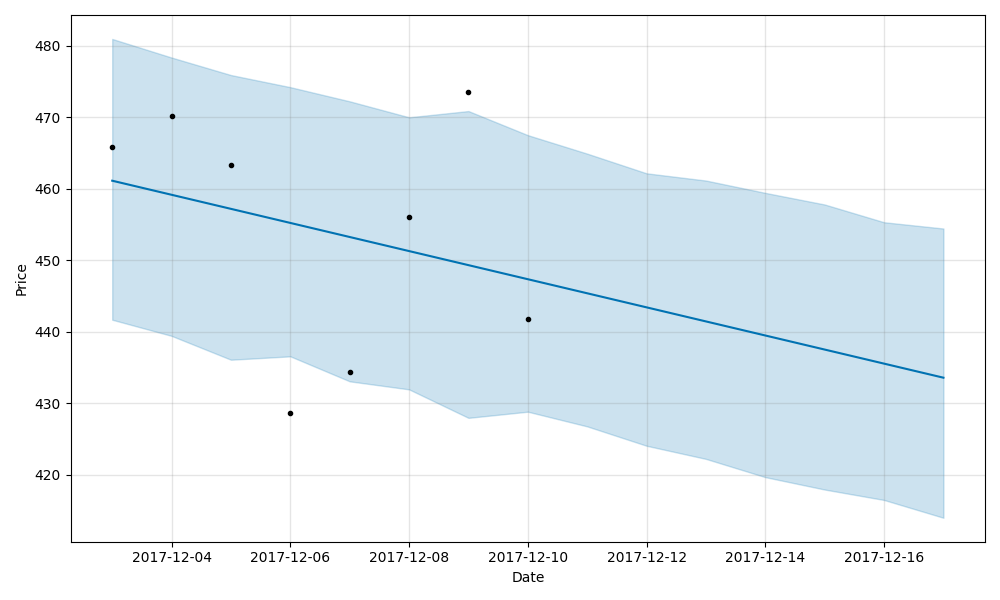
\includegraphics[width=0.5\textwidth]{./plots/prophet/eth/week/9}}
   \subfloat[]{
   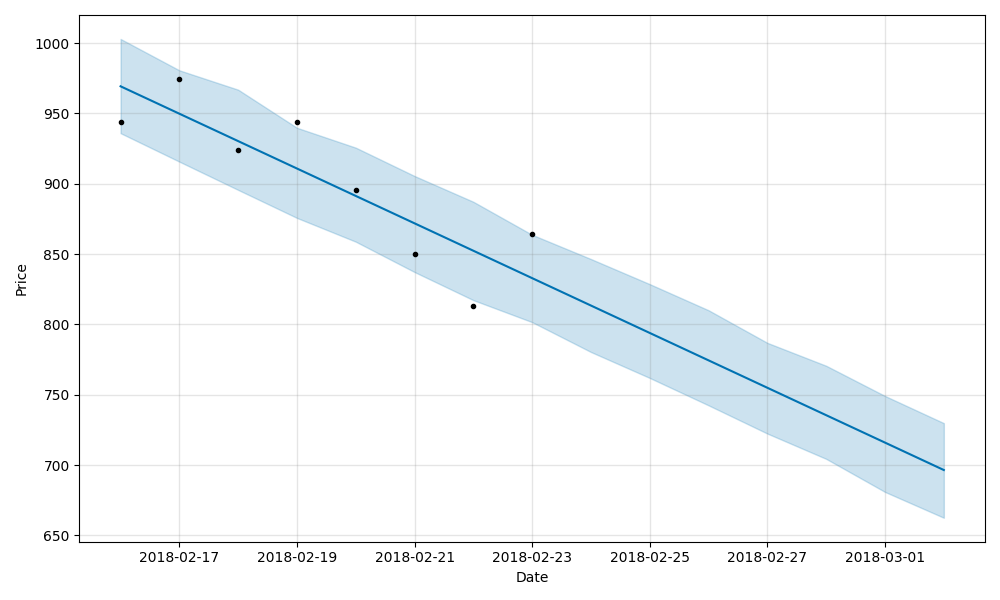
\includegraphics[width=0.5\textwidth]{./plots/prophet/eth/week/10}}
  \caption{Predicción del modelo entrenado con 10 semanas aleatorias de ETH}
  \label{f:eth_wk_prophet}
\end{figure}

\begin{table}[h!]
 \begin{center}
  \begin{tabular}{|r|c|c|c|c|c|c|c|c|c|c|}
    Métrica & (a) & (b) & (c) & (d) & (e) & (f) & (g) & (h) & (i) & (j) \\ \hline
    MAE & 26.32 & 1815 & 355.1 & 137.0 & 93.29 & 36.97& 1234& 20.45 & 493.7 & 410.3 \\
    RMSE & 26.32 & 1815 & 355.1 & 137.0 & 93.29 & 36.97& 1234& 20.45 & 493.7 & 410.3 \\
    MAPE & 0.154 & 0.452 & 0.089 & 0.485 & 0.164 & 0.054 & 0.340 & 0.108 & 0.144 & 0.106 \\ \hline
  \end{tabular}
  \caption{Métricas de la figura \ref{f:eth_wk_prophet}}
  \label{tab:eth_prophet_wk}
 \end{center}
\end{table}

\begin{figure}
 \centering
  \subfloat[]{
   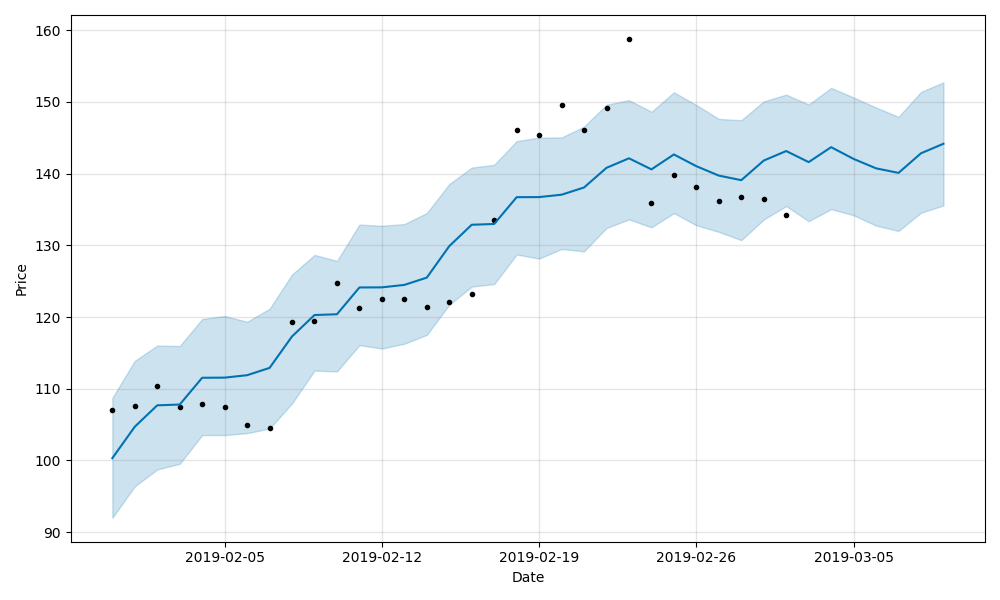
\includegraphics[width=0.5\textwidth]{./plots/prophet/eth/month/1}}
  \subfloat[]{
   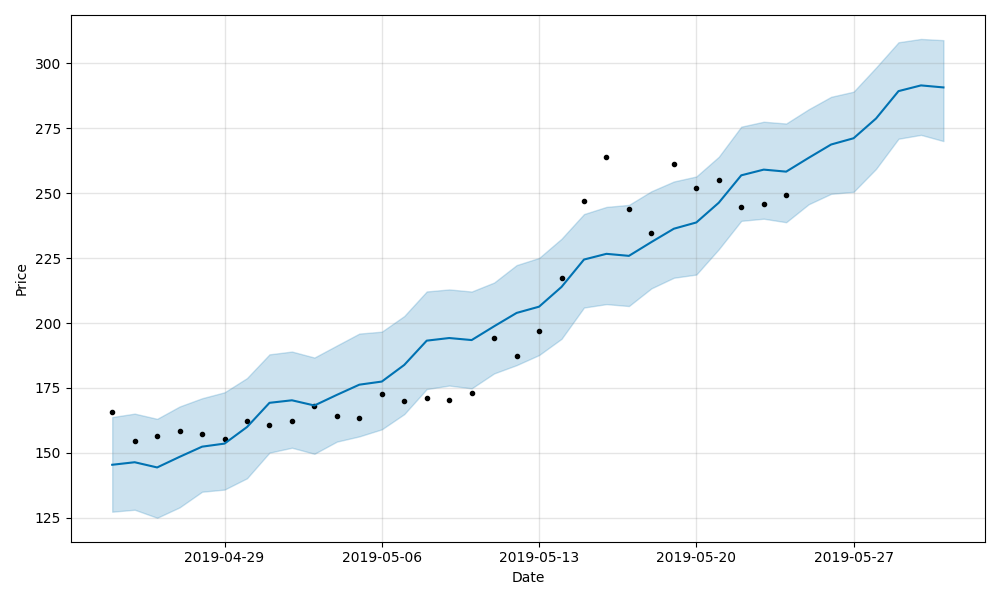
\includegraphics[width=0.5\textwidth]{./plots/prophet/eth/month/2}} \\
  \subfloat[]{
   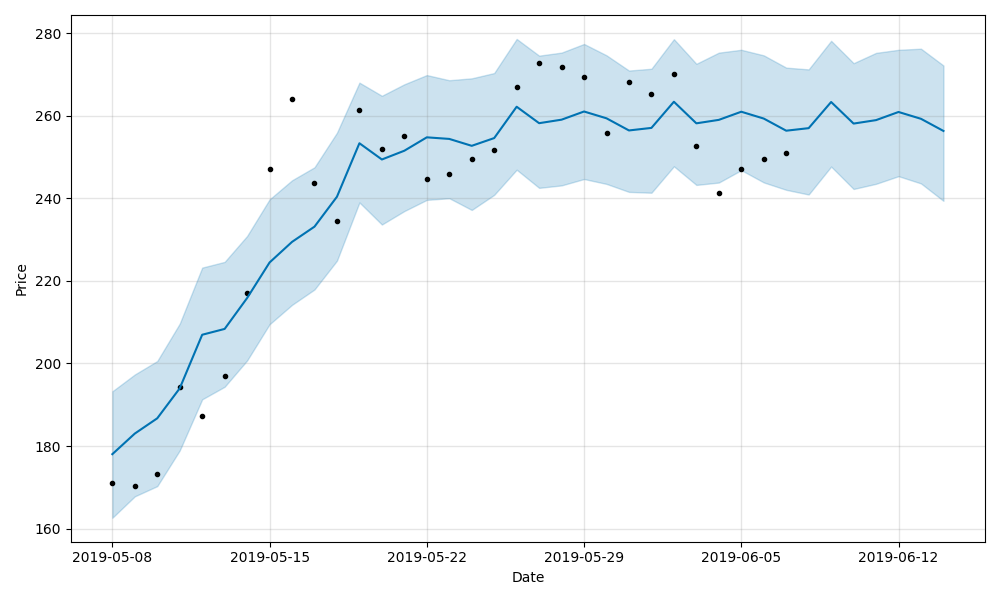
\includegraphics[width=0.5\textwidth]{./plots/prophet/eth/month/3}}
   \subfloat[]{
   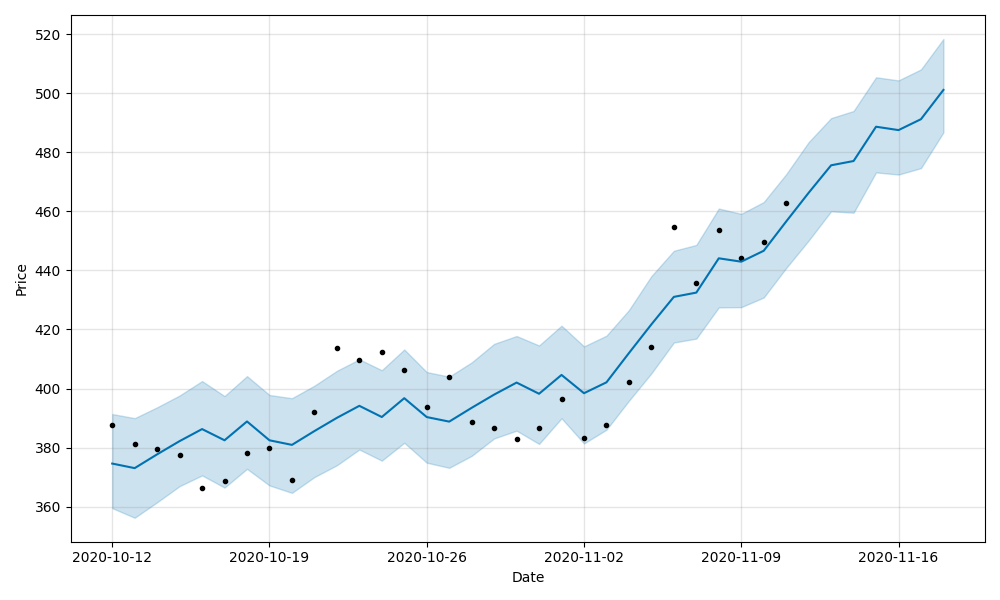
\includegraphics[width=0.5\textwidth]{./plots/prophet/eth/month/4}} \\
   \subfloat[]{
   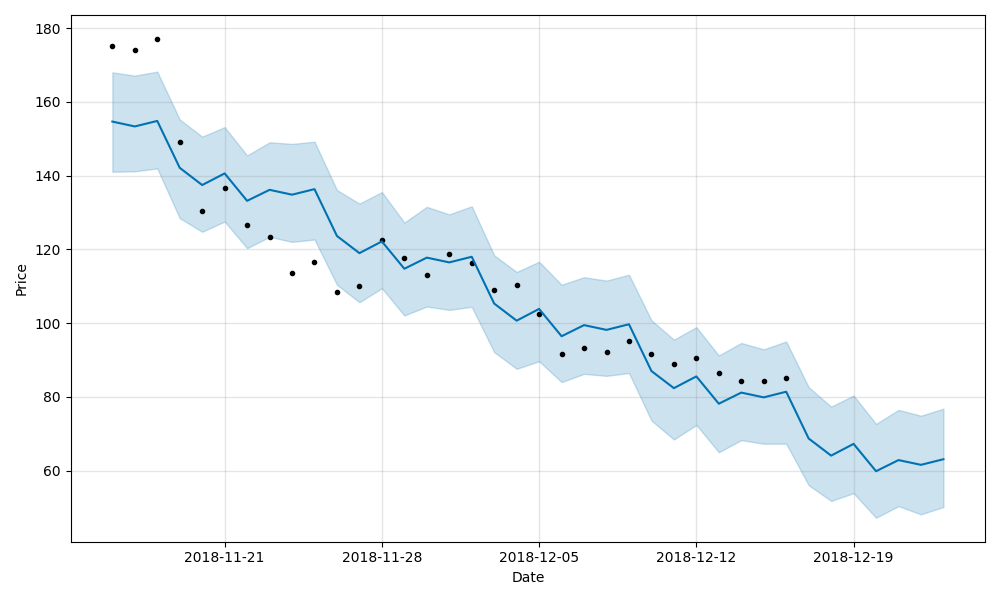
\includegraphics[width=0.5\textwidth]{./plots/prophet/eth/month/5}}
   \subfloat[]{
   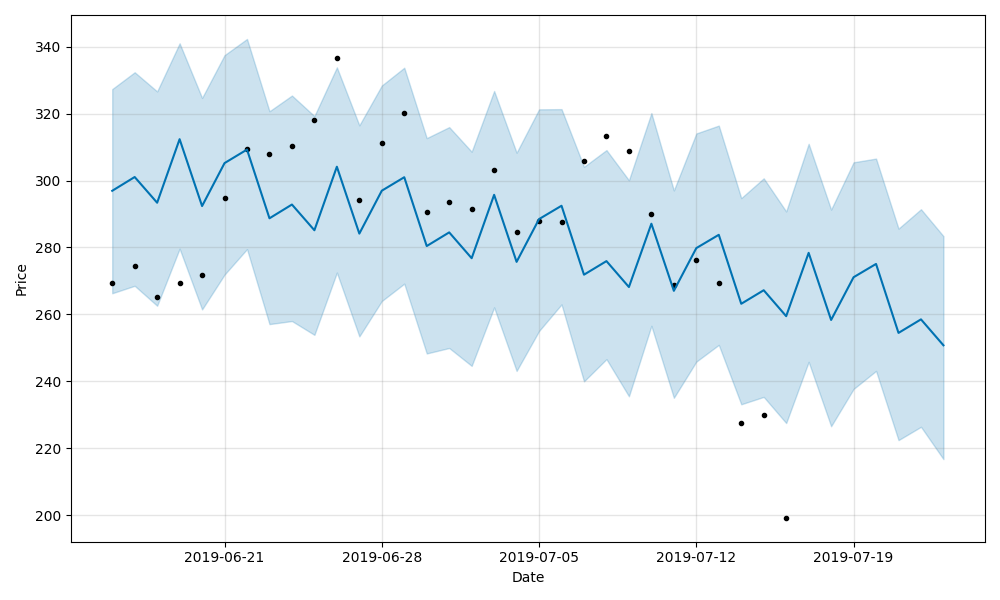
\includegraphics[width=0.5\textwidth]{./plots/prophet/eth/month/6}} \\
   \subfloat[]{
   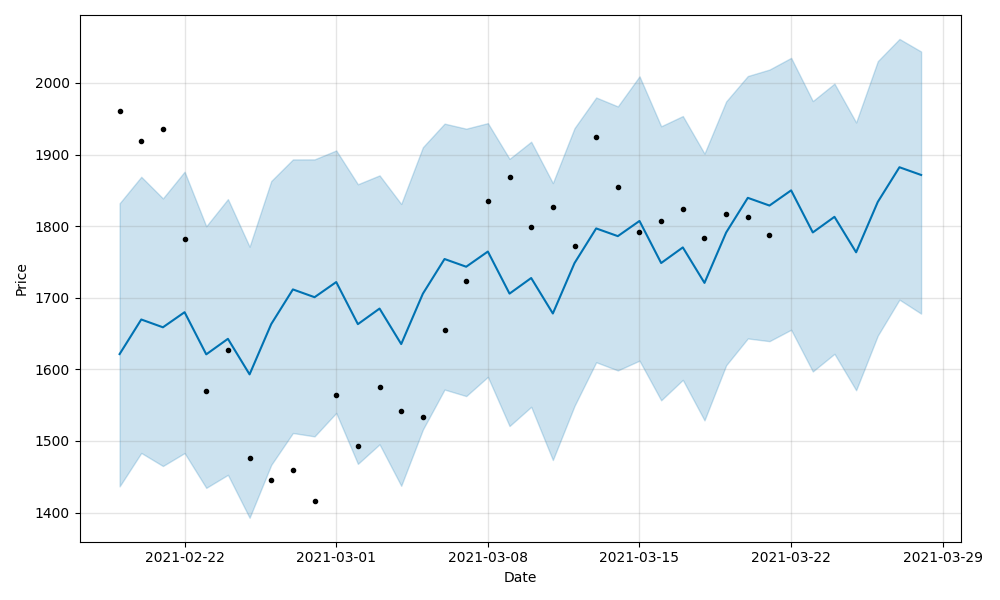
\includegraphics[width=0.5\textwidth]{./plots/prophet/eth/month/7}}
   \subfloat[]{
   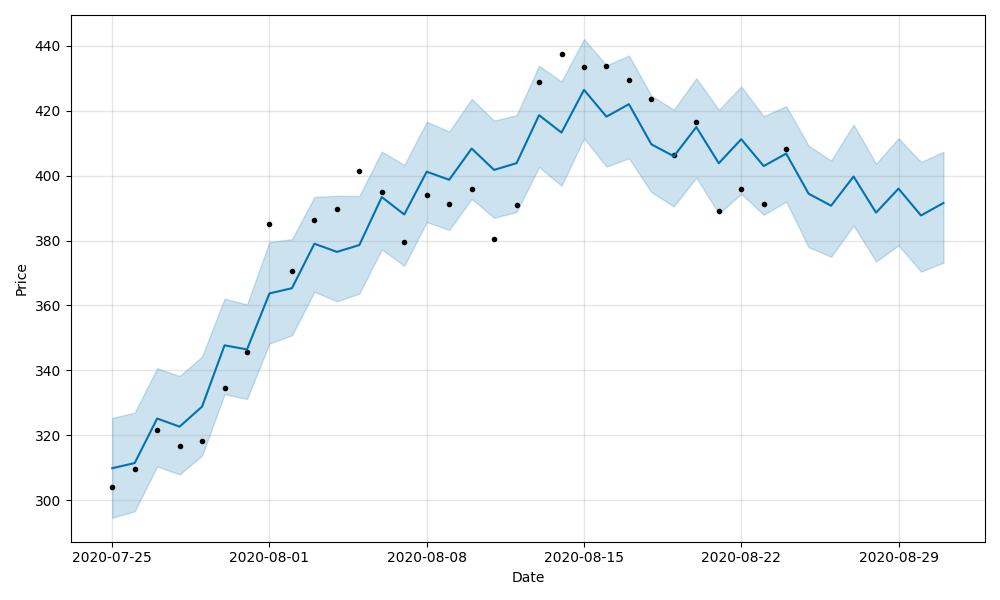
\includegraphics[width=0.5\textwidth]{./plots/prophet/eth/month/8}} \\
   \subfloat[]{
   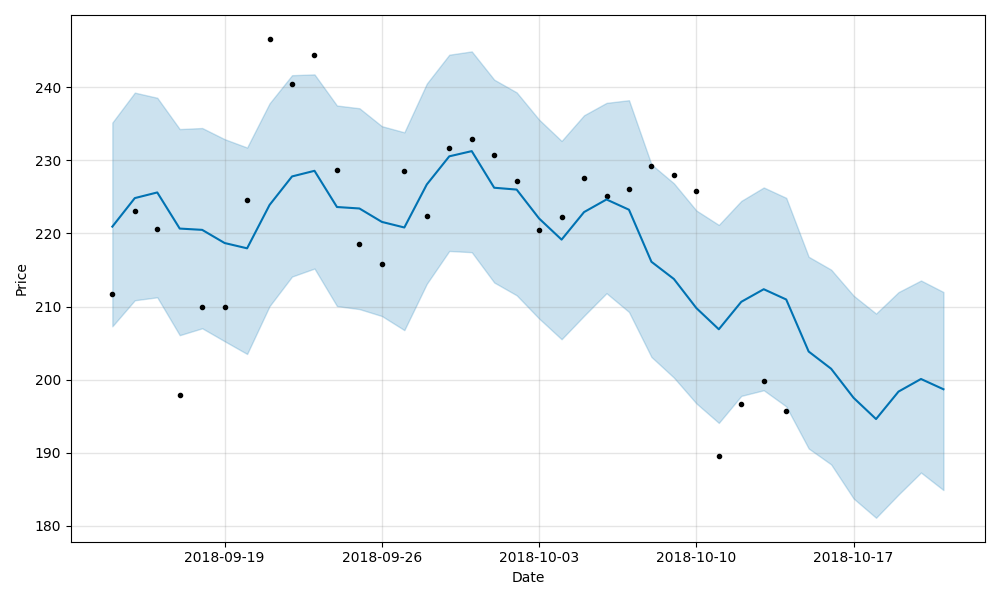
\includegraphics[width=0.5\textwidth]{./plots/prophet/eth/month/9}}
   \subfloat[]{
   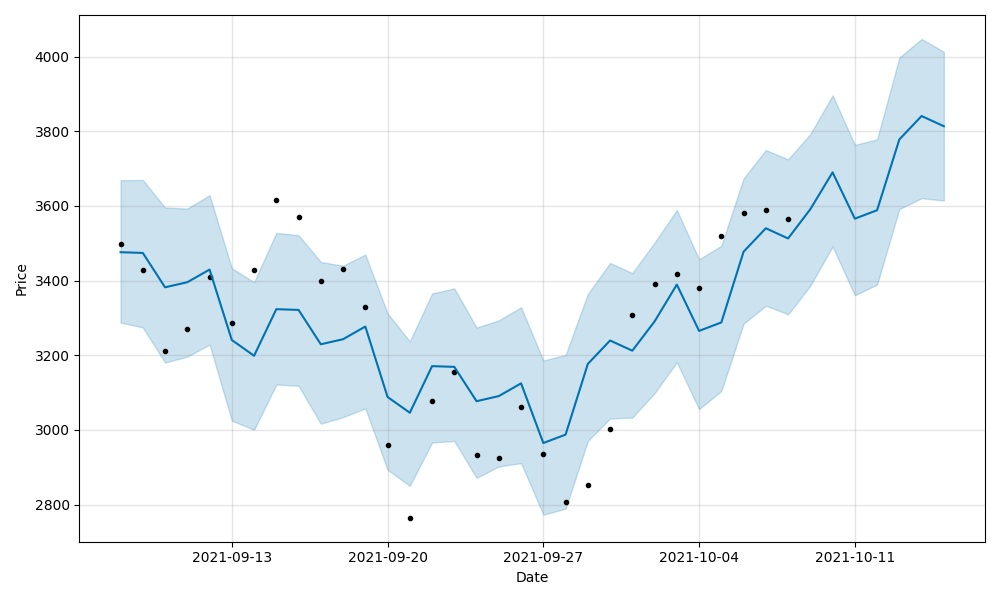
\includegraphics[width=0.5\textwidth]{./plots/prophet/eth/month/10}}
  \caption{Predicción del modelo entrenado con 10 meses aleatorios de ETH}
  \label{f:eth_mth_prophet}
\end{figure}

\begin{table}[t]
 \begin{center}
  \begin{tabular}{|r|c|c|c|c|c|c|c|c|c|c|}
    Métrica & (a) & (b) & (c) & (d) & (e) & (f) & (g) & (h) & (i) & (j) \\ \hline
    MAE  & 250.6 & 201.6 & 364.2 & 19618 & 557.8 & 2882 & 401.7 & 1355 & 3486 & 68112 \\
    RMSE & 336.3 & 242.7 & 476.9 & 27536 & 779.5 & 4009 & 509.8 & 1879 & 4907 & 95783 \\
    MAPE & 1.809 & 1.171 & 1.385 & 10.81 & 4.934 & 9.370 & 0.963 & 3.650 & 14.51 & 19.07 \\ \hline
  \end{tabular}
  \caption{Métricas de la figura \ref{f:eth_mth_prophet}}
  \label{tab:eth_prophet_m}
 \end{center}
\end{table}

\begin{figure}[h!]
 \centering
  \subfloat[]{
   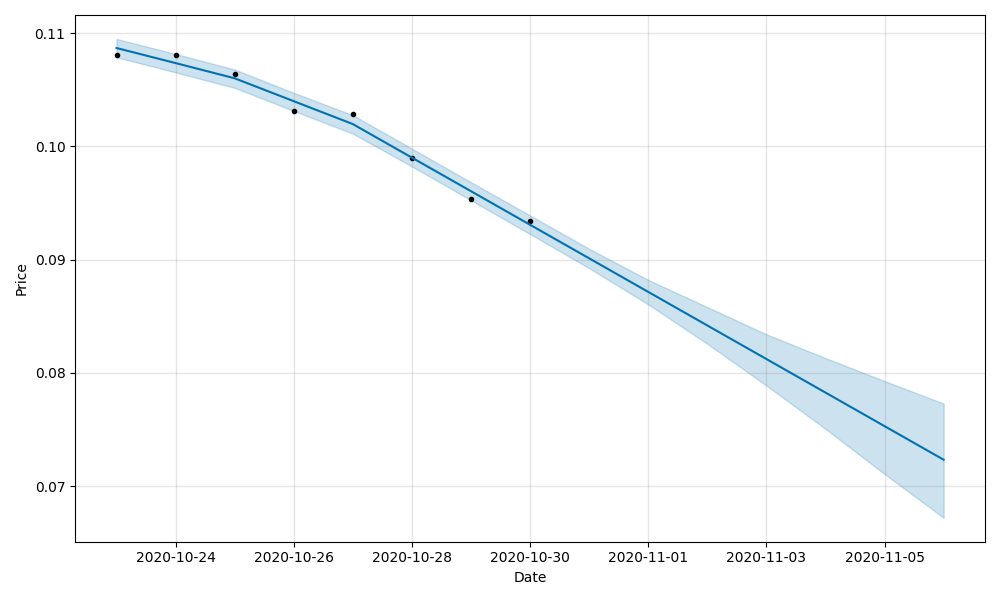
\includegraphics[width=0.5\textwidth]{./plots/prophet/ada/week/1}}
  \subfloat[]{
   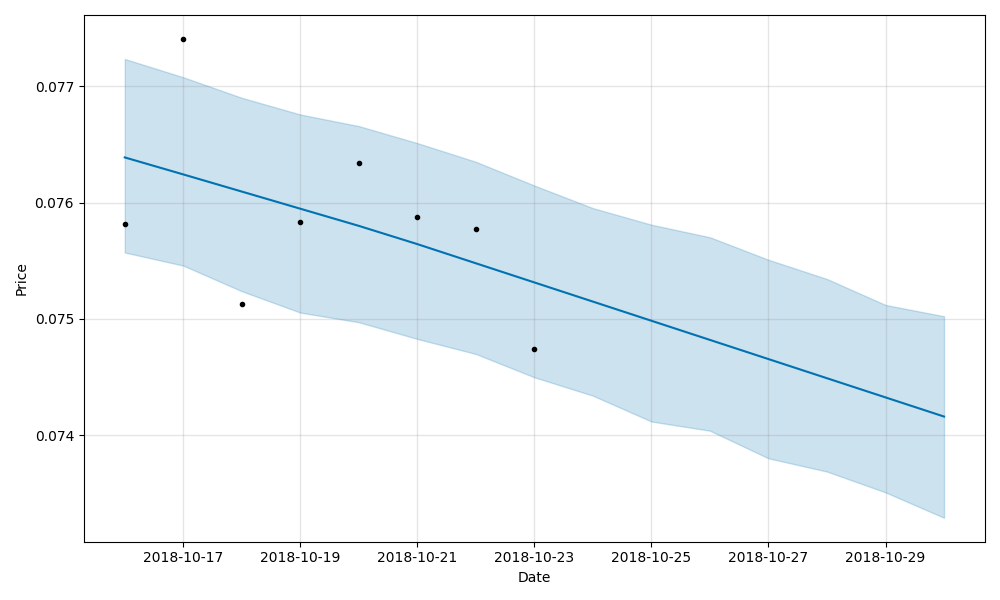
\includegraphics[width=0.5\textwidth]{./plots/prophet/ada/week/2}} \\
  \subfloat[]{
   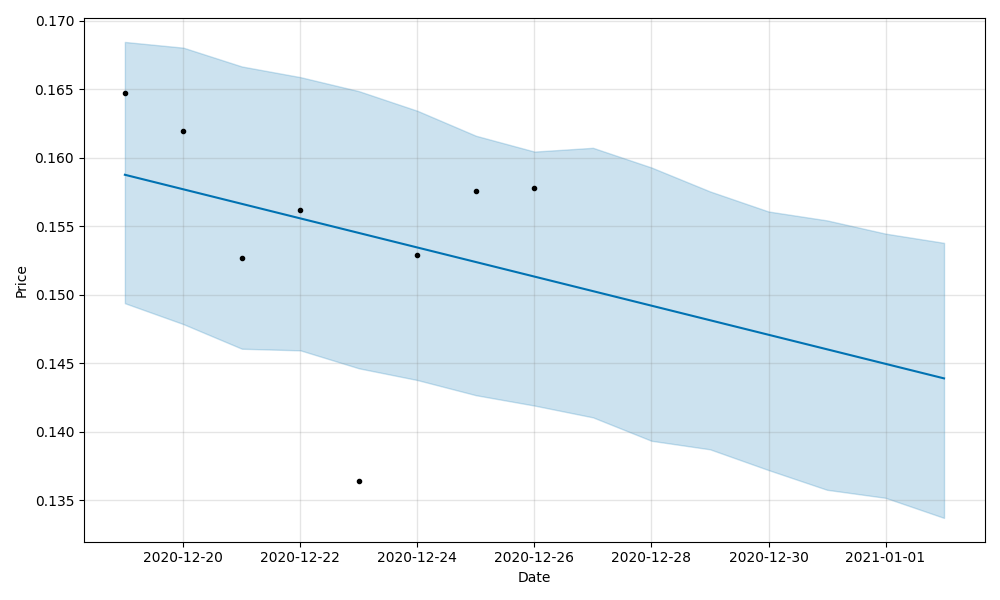
\includegraphics[width=0.5\textwidth]{./plots/prophet/ada/week/3}}
   \subfloat[]{
   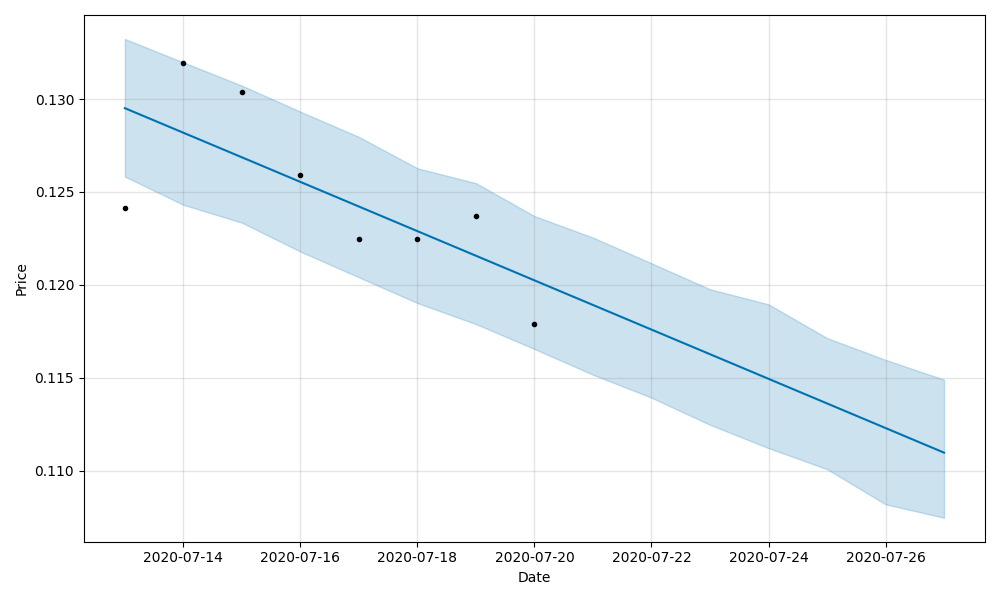
\includegraphics[width=0.5\textwidth]{./plots/prophet/ada/week/4}} \\
   \subfloat[]{
   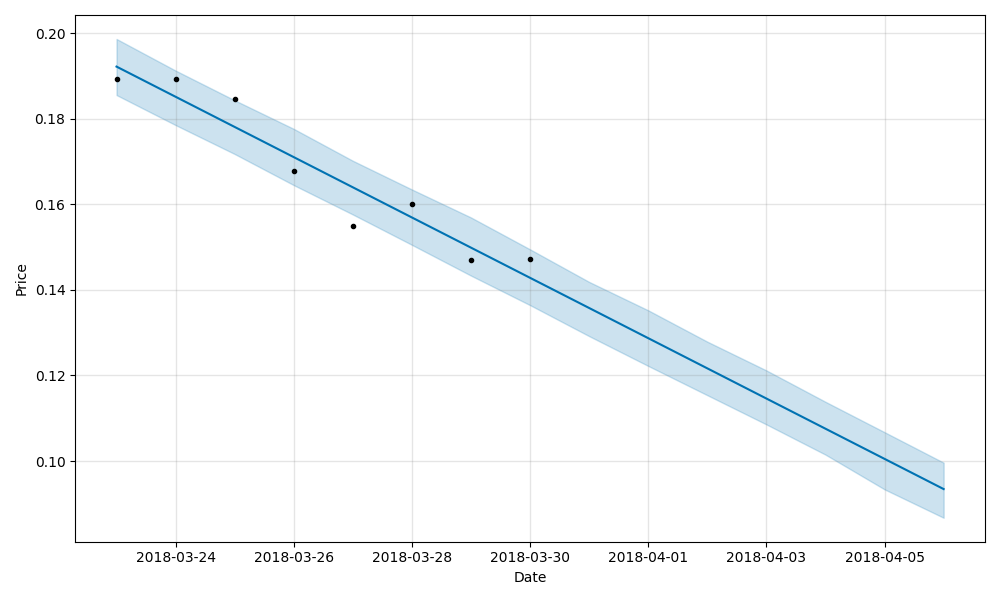
\includegraphics[width=0.5\textwidth]{./plots/prophet/ada/week/5}}
   \subfloat[]{
   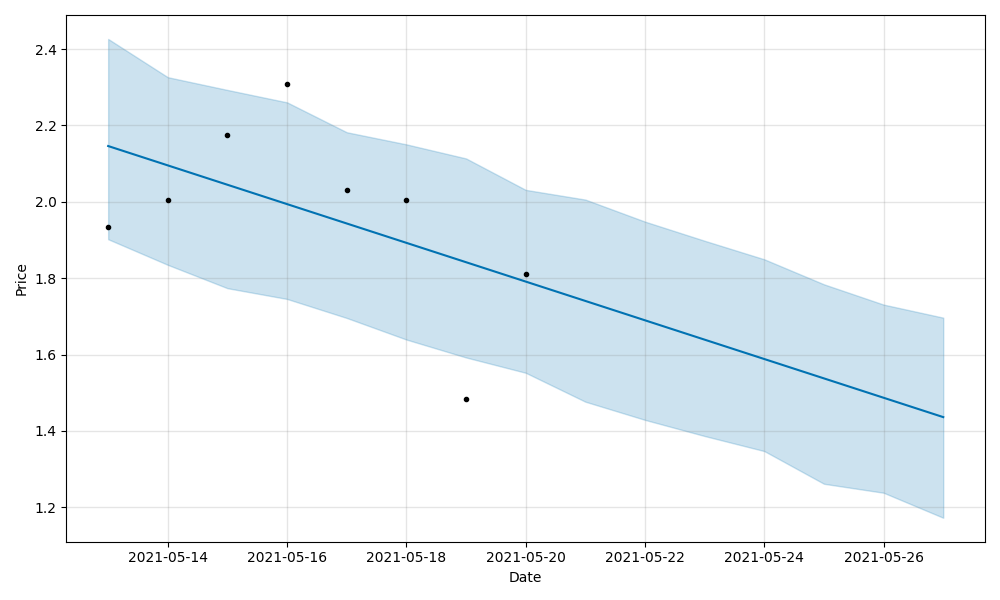
\includegraphics[width=0.5\textwidth]{./plots/prophet/ada/week/6}} \\
   \subfloat[]{
   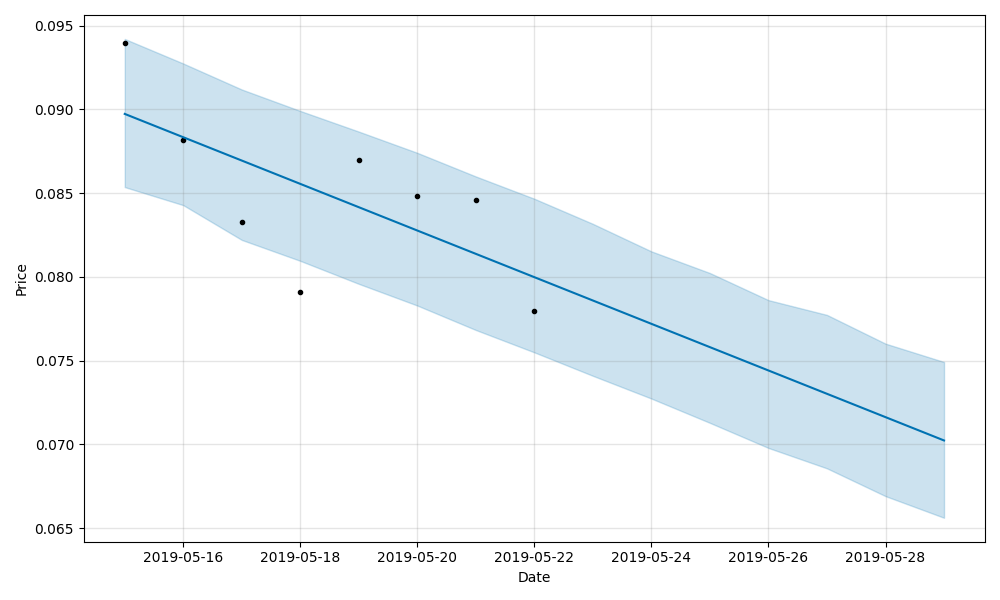
\includegraphics[width=0.5\textwidth]{./plots/prophet/ada/week/7}}
   \subfloat[]{
   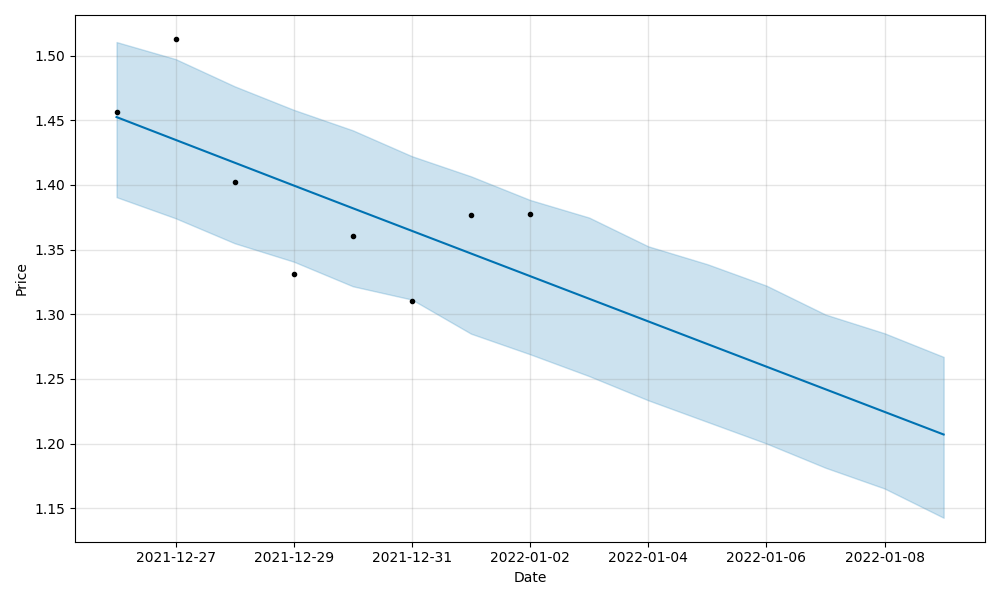
\includegraphics[width=0.5\textwidth]{./plots/prophet/ada/week/8}} \\
   \subfloat[]{
   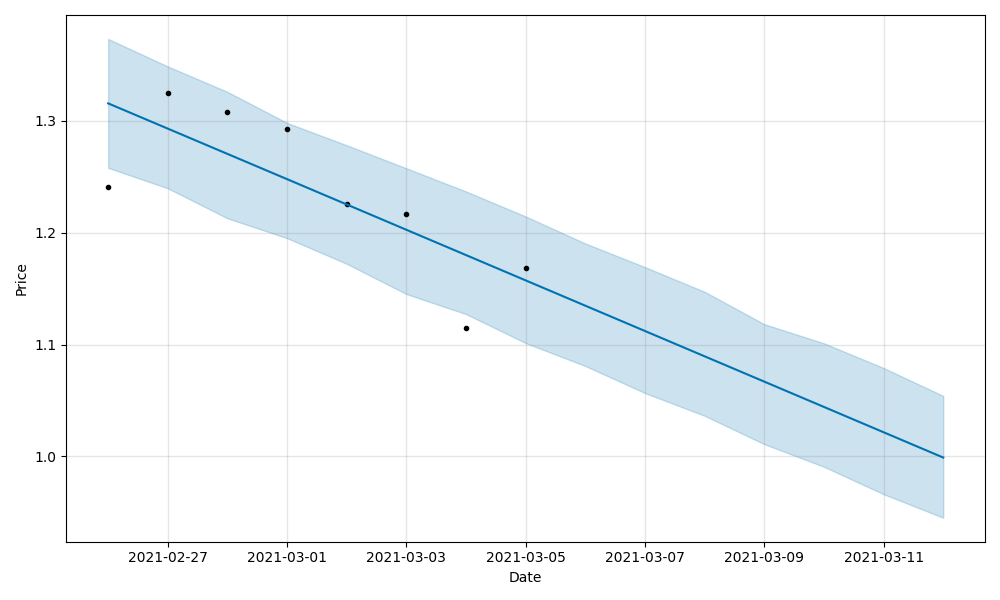
\includegraphics[width=0.5\textwidth]{./plots/prophet/ada/week/9}}
   \subfloat[]{
   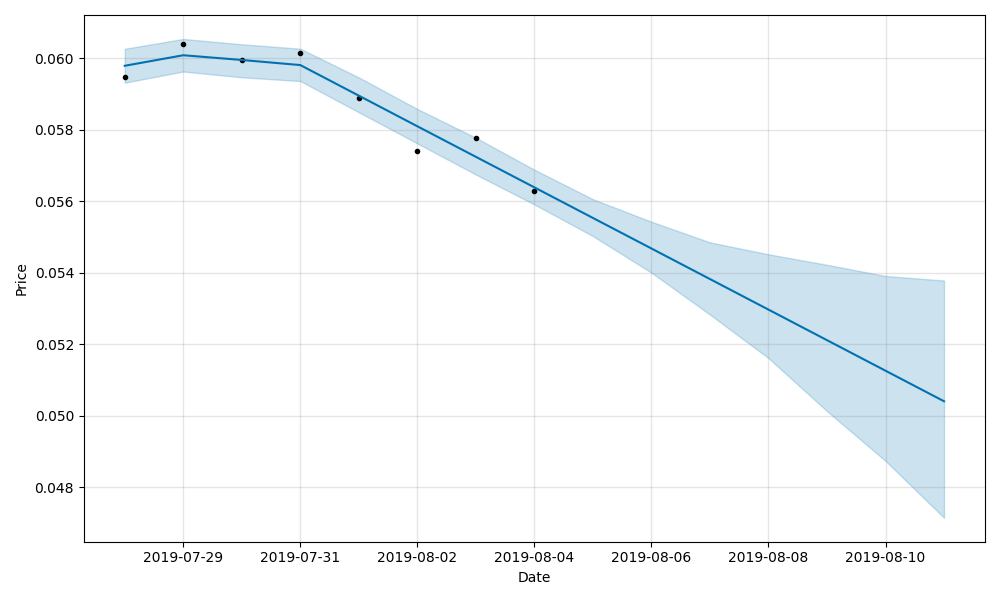
\includegraphics[width=0.5\textwidth]{./plots/prophet/ada/week/10}}
  \caption{Predicción del modelo entrenado con 10 semanas aleatorias de ADA}
  \label{f:ada_wk_prophet}
\end{figure}

\begin{table}[h!]
 \begin{center}
  \begin{tabular}{|r|c|c|c|c|c|c|c|c|c|c|}
    Métrica & (a) & (b) & (c) & (d) & (e) & (f) & (g) & (h) & (i) & (j) \\ \hline
    MAE & 0.001 & 0.020 & 0.183 & 0.008 & 0.041 & 0.621 & 0.024 & 0.476 & 0.658 & 0.015 \\
    RMSE & 0.001 & 0.020 & 0.183 & 0.008 & 0.041 & 0.621 & 0.024 & 0.476 & 0.658 & 0.015 \\
    MAPE & 0.009 & 0.336 & 1.553 & 0.094 & 0.282 & 0.343 & 0.314 & 0.345 & 0.563 & 0.091 \\ \hline
  \end{tabular}
  \caption{Métricas de la figura \ref{f:ada_wk_prophet}}
  \label{tab:ada_prophet_wk}
 \end{center}
\end{table}

\begin{figure}
 \centering
  \subfloat[]{
   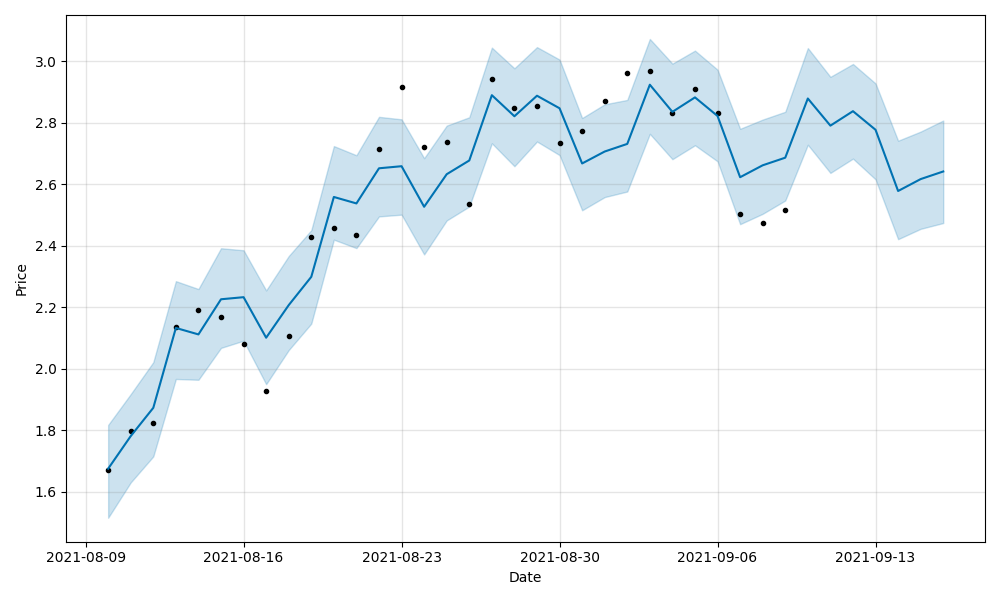
\includegraphics[width=0.5\textwidth]{./plots/prophet/ada/month/1}}
  \subfloat[]{
   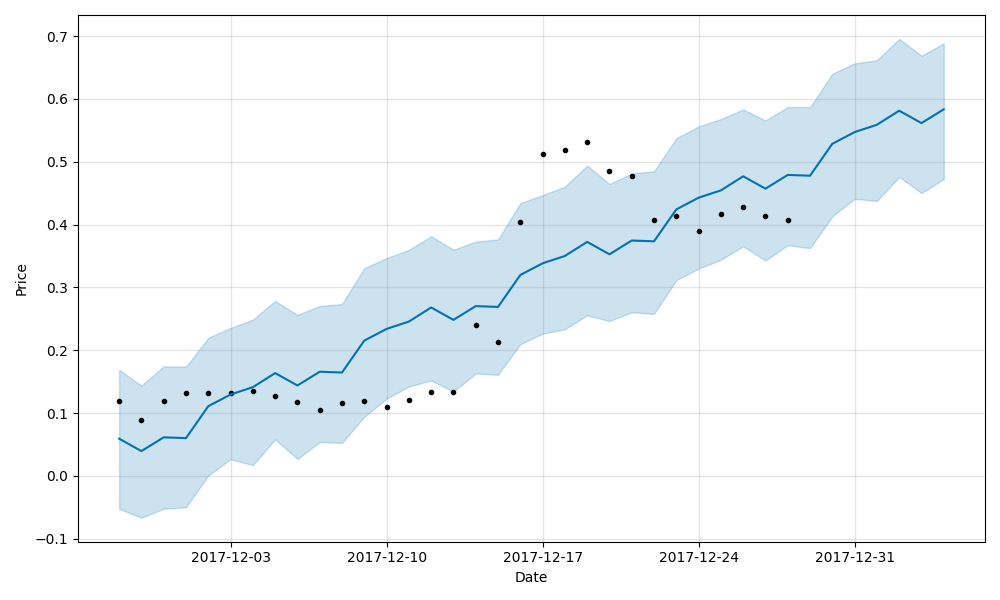
\includegraphics[width=0.5\textwidth]{./plots/prophet/ada/month/2}} \\
  \subfloat[]{
   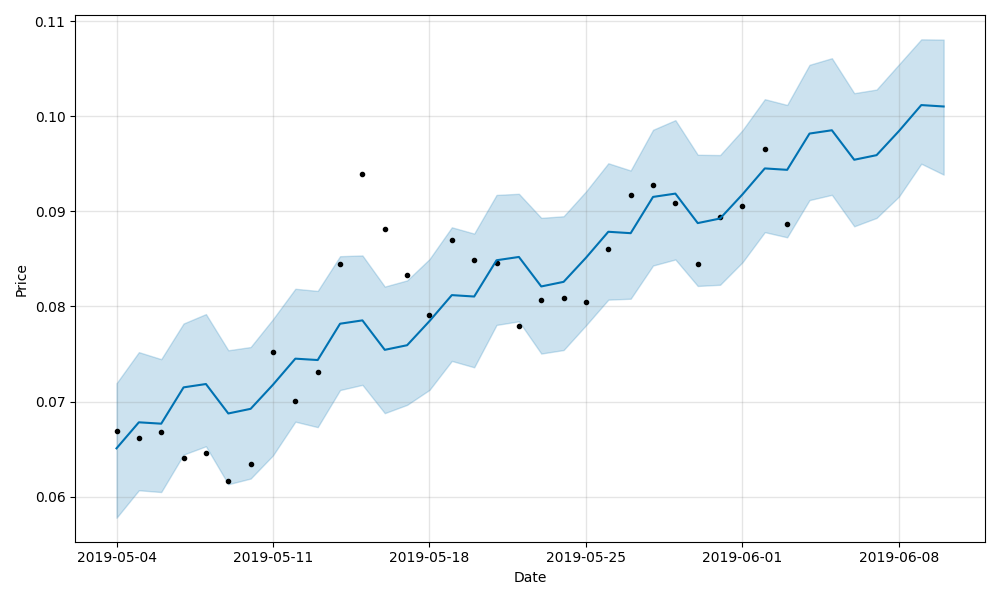
\includegraphics[width=0.5\textwidth]{./plots/prophet/ada/month/3}}
   \subfloat[]{
   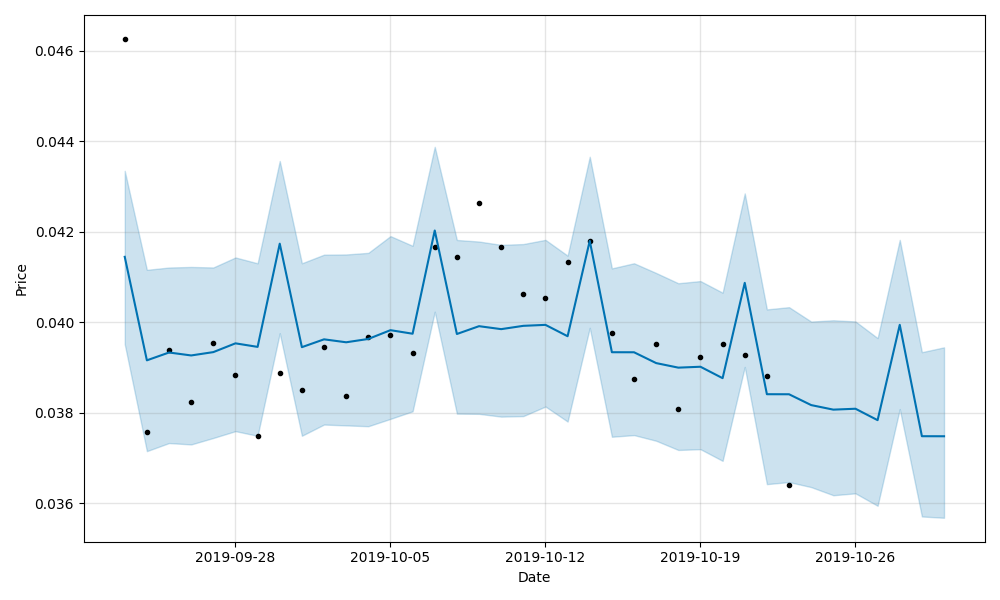
\includegraphics[width=0.5\textwidth]{./plots/prophet/ada/month/4}} \\
   \subfloat[]{
   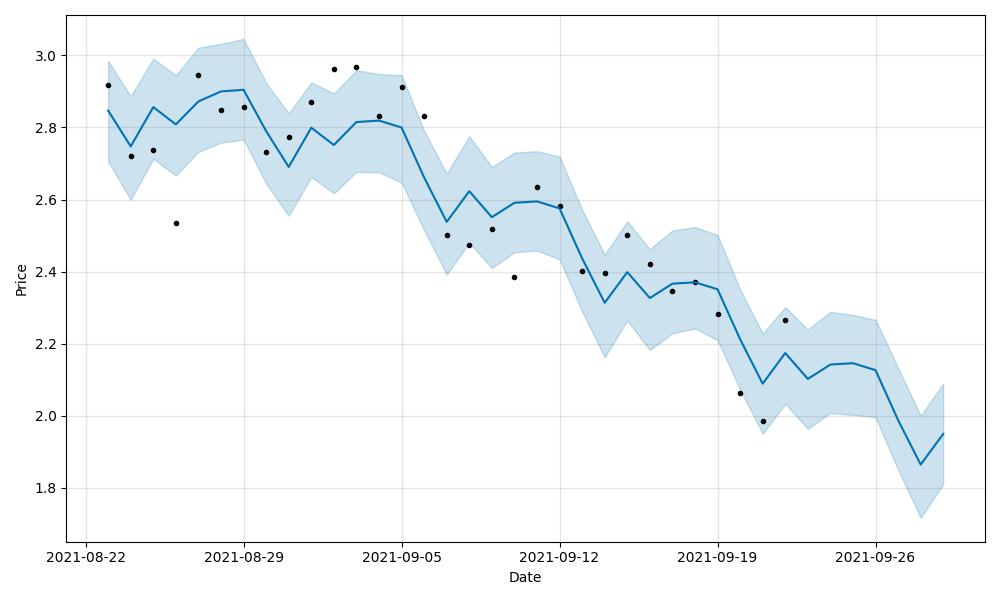
\includegraphics[width=0.5\textwidth]{./plots/prophet/ada/month/5}}
   \subfloat[]{
   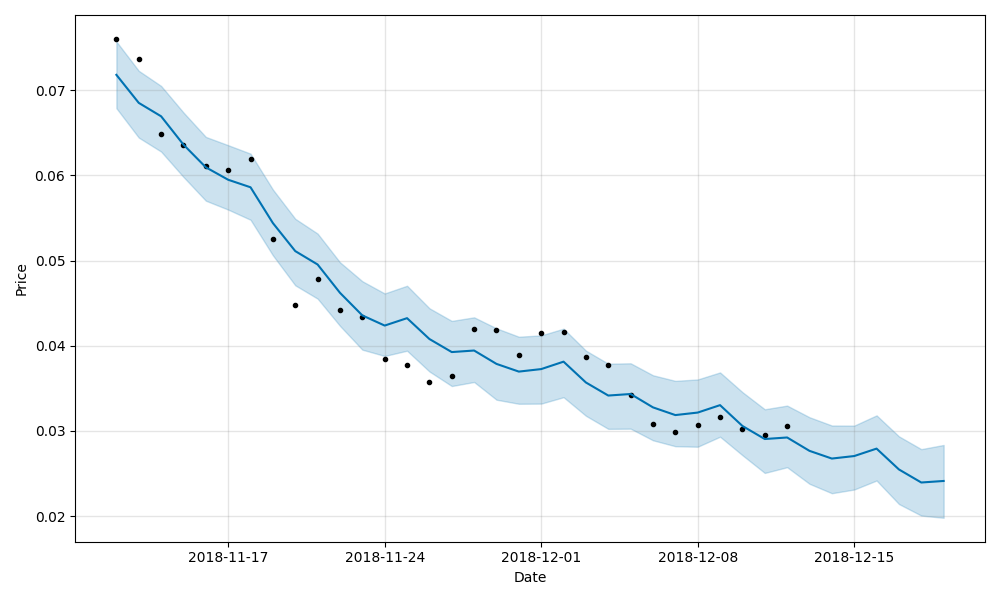
\includegraphics[width=0.5\textwidth]{./plots/prophet/ada/month/6}} \\
   \subfloat[]{
   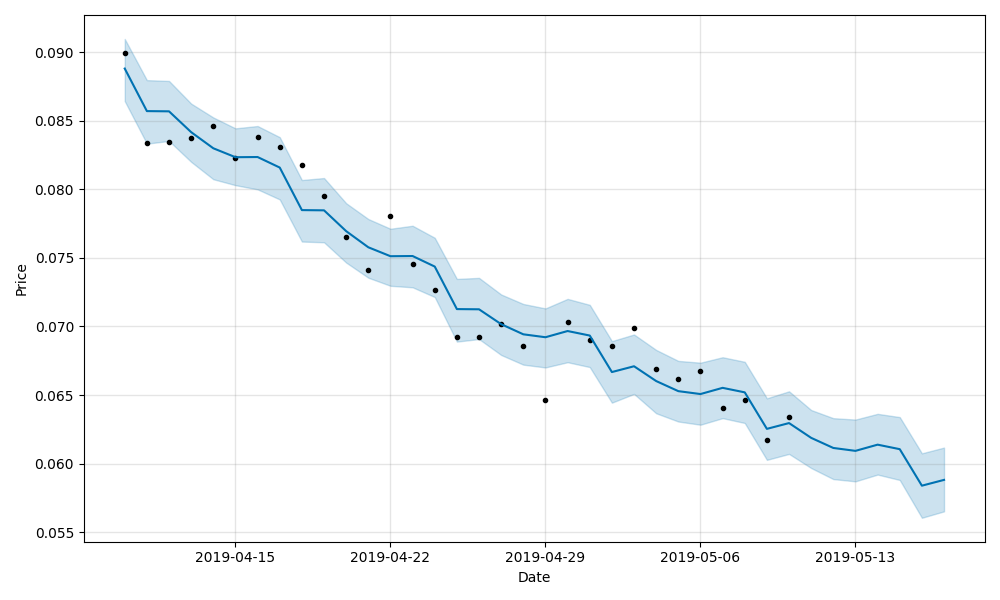
\includegraphics[width=0.5\textwidth]{./plots/prophet/ada/month/7}}
   \subfloat[]{
   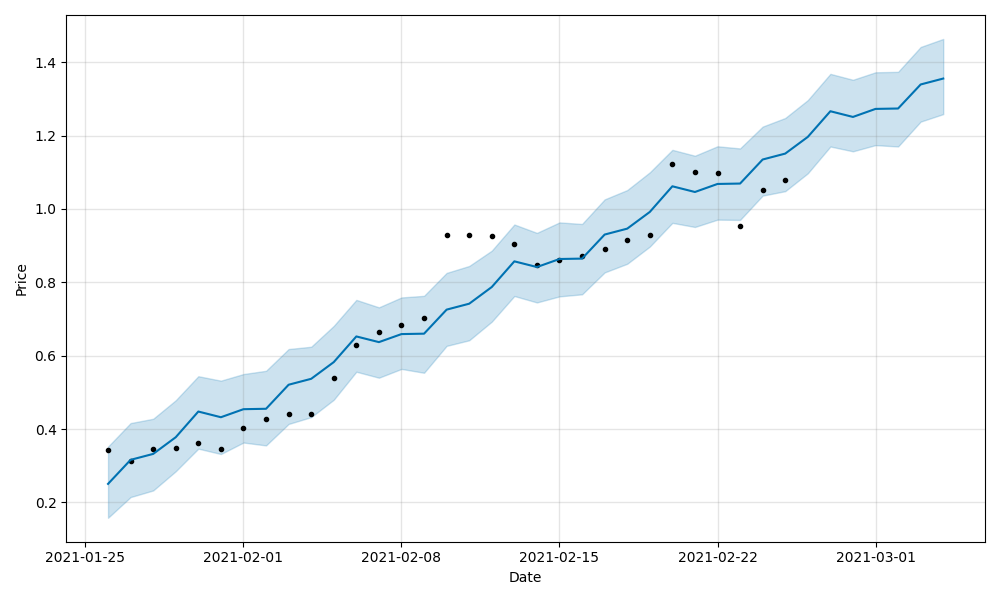
\includegraphics[width=0.5\textwidth]{./plots/prophet/ada/month/8}} \\
   \subfloat[]{
   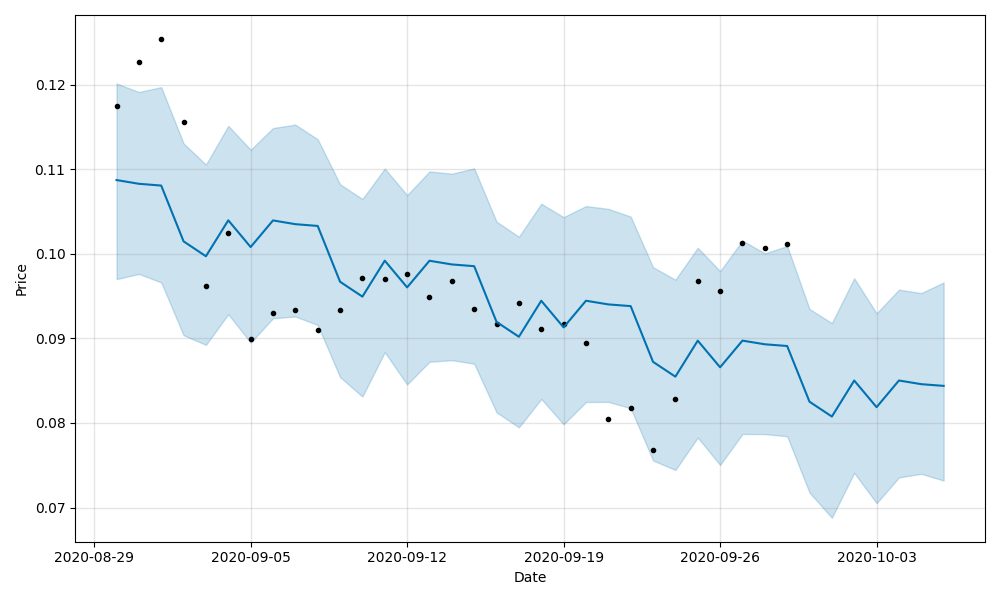
\includegraphics[width=0.5\textwidth]{./plots/prophet/ada/month/9}}
   \subfloat[]{
   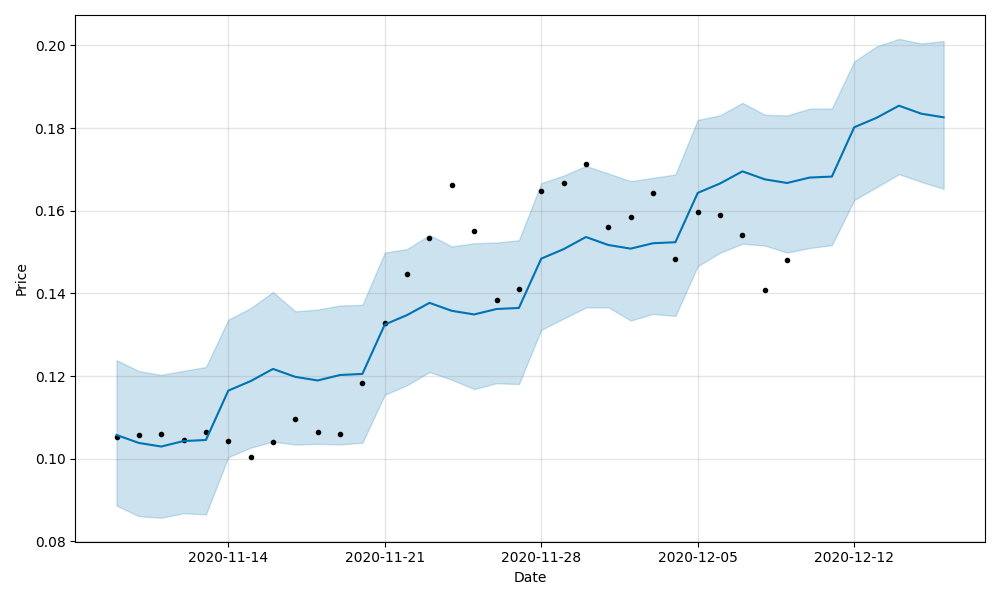
\includegraphics[width=0.5\textwidth]{./plots/prophet/ada/month/10}}
  \caption{Predicción del modelo entrenado con 10 meses aleatorios de ADA}
  \label{f:ada_mth_prophet}
\end{figure}

\begin{table}[t]
 \begin{center}
  \begin{tabular}{|r|c|c|c|c|c|c|c|c|c|c|}
    Métrica & (a) & (b) & (c) & (d) & (e) & (f) & (g) & (h) & (i) & (j) \\ \hline
    MAE & 0.354 & 23.34 & 0.085 & 0.011 & 14.69 & 0.176 & 0.673 & 0.150 & 0.215 & 0.227 \\
    RMSE & 0.495 & 32.89 & 0.114 & 0.012 & 20.74 & 0.242 & 0.476 & 0.211 & 0.295 & 0.294 \\
    MAPE & 11.83 & 14.38 & 1.204 & 0.291 & 5.300 & 4.000 & 5.823 & 4.354 & 1.023 & 2.027 \\ \hline
  \end{tabular}
  \caption{Métricas de la figura \ref{f:ada_mth_prophet}}
  \label{tab:ada_prophet_m}
 \end{center}
\end{table}

\end{document}
